\documentclass[pdftex,12pt,a4paper]{article}

\usepackage{wrapfig, amssymb, amsmath, graphicx, subfigure, pifont, seqsplit, float, booktabs, siunitx, adjustbox}
\usepackage[english]{babel}
\usepackage[top=1in, bottom=1in, left=1in, right=1in]{geometry}
\pagenumbering{arabic}
\newcommand{\HRule}{\rule{\linewidth}{0.5mm}}

\usepackage{forest}
\tikzset{el style/.style={midway, font=\scriptsize, inner sep=+1pt, auto=right}}
\forestset{angled/.style={
    content/.expanded={\noexpand\textless\forestov{content}\noexpand\textgreater}}}

\begin{document}
\begin{titlepage}

% Upper part of the page
\begin{flushleft}

\includegraphics[trim=0mm 0mm 0mm 0mm, width=1\textwidth]{./logo.jpg}\\
\end{flushleft}
\begin{center}
	\textsc{\Large Informatie en Communicatie}\\[0.5cm]

    % Title
    \HRule \\[0.4cm] { \huge \bfseries HW-1}\\[0.4cm]

    \HRule \\[1.5cm]

    % Author and supervisor
\begin{minipage}{0.4\textwidth}
\begin{flushleft} \large \emph{Authors:}\\
Abe \textsc{Wiersma}\\
\end{flushleft}
\end{minipage}
\begin{minipage}{0.4\textwidth} \begin{flushright} \large \end{flushright}\end{minipage}

    \vfill

    % Bottom of the page 
    {\large \today}

\end{center}
\end{titlepage}
\pagebreak

\begin{enumerate}
    \item Let $X$ be a discrete random variable.  Show that the entropy of a
        function $g$ of $X$ is less than or equal to the entropy of $X$ by
        justifying the following steps:
        \begin{align}
            \intertext{$H[g(X)|X] = 0$ the value of g(X) is completely determined by the value of X.}
            H(X) &= H(X) + H[g(X)|X]\\
            \intertext{$H(g(X)|X)=H(X,g(X))-H(X)$ Shannon Entropy conditional chain rule}
                 &= H(X,g(X))\\
            \intertext{H(X,g(X)) = H(g(X),X)), apply Shannon Entropy conditional chain rule again, $H(g(X),X)=H(X|g(X))+H(g(X))$}
                 &= H(g(X)) + H(X|g(X))\\
            \intertext{$H(g(X)) + H(X|g(X)) \ge H(g(X))$
                       \textbf{Proposition 4[CF]:} $\implies H(X|g(X)) \ge 0 $}
                 &\ge H(g(X))
        \end{align}

    \item Let $X$ and $Y$ be independent binary random variables with:
        $$P_X[1] = P_X[0] = P_Y[1] = P_Y[0] = \frac{1}{2}$$
        Compute H(X+Y).
        \begin{align}
               Z &= X+Y\\
            p(Z) &= \begin{cases}
                        \frac{1}{4} & Z= 0\\
                        \frac{1}{2} & Z= 1\\
                        \frac{1}{4} & Z= 2
                    \end{cases}\\
         H(Z) &= -\left(\sum_{z \in Z}{P(z) \log P(z)}\right)\\
              &= -\left(\frac{1}{4}log\left(\frac{1}{4}\right)
                       +\frac{1}{2}log\left(\frac{1}{2}\right)
                       +\frac{1}{4}log\left(\frac{1}{4}\right)\right)\\
              &= 1.5
        \end{align}
    \newpage
    \item Use Jensen's inequality to derive an inequality between $E[X^2]$ and
        $E[X]^2$. Use this inequality as an alternative proof that
        $Var[X] \ge 0$.
        \begin{align}
            \intertext{\textbf{Proposition 2.} Jensen's inequality}
            E\left[f(X)\right] &\geq f\left(E[X]\right)\\
            \intertext{Define $f(x)$}
            f(x) &= x^2
            \intertext{Apply Jensen's inequality}
            E\left[X^2\right] &\geq \left(E[X]\right)^2
            \intertext{Show $Var[X] \ge 0$}
            E\left[X^2\right] - \left(E[X]\right)^2 &\ge 0\\
            Var[X] &\ge 0
        \end{align}
    \item The mutual information between two random variables $X$ and $Y$ is
        defined as $I(X;Y) := H(X) - H(X|Y)$
        \begin{enumerate}
            \item Show that the mutual information can be expressed in terms of
                the relative entropy, i.e. that $I(X;Y) =D_{KL}(P_{XY}||P_XP_Y)$
                % \begin{center}
                %     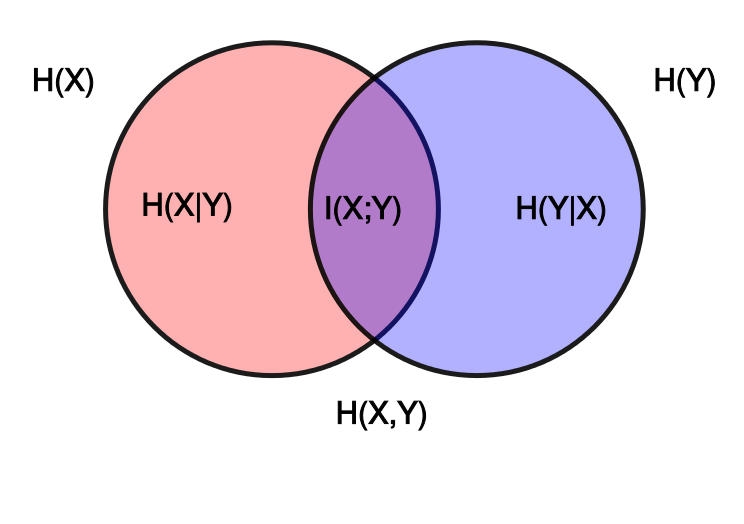
\includegraphics[width=0.6\textwidth]{venn.png}
                % \end{center}
                \begin{align}
                    I(X;Y) &= H(X) - H(X|Y)\\
                           &= -\sum_{x \in X} {P_X(x) \log P_X(x)}-\sum_{x \in X,y \in Y}P_{XY}(x,y)\log\frac{P_Y(y)}{P_{XY}(x,y)}\\
                           &= - \sum_{x \in X}\sum_{y\in Y} P_X(x) P_{XY}(y|x)\log P_X(x)-\sum_{x \in X}\sum_{y\in Y} P_{XY}(x,y) \log\frac{P_Y(y)}{P_{XY}(x,y)}\\
                           &= -\sum_{x \in X}\sum_{y\in Y} P_{XY}(x,y) \log\frac{P_Y(y)}{P_{XY}(x,y)} - \sum_{x \in X}\sum_{y\in Y} P_{XY}(x,y)\log P_X(x)\\
                           &= \sum_{x \in X}\sum_{y\in Y} P_{XY}(x,y) \left(-\log\frac{P_Y(y)}{P_{XY}(x,y)} - \log P_X(x))\right)\\
                           &= \sum_{x \in X}\sum_{y\in Y} P_{XY}(x,y) (\log P_{XY}(x,y) - (\log P_X(x) + \log P_Y(y)))\\
                           &= \sum_{x \in X}\sum_{y\in Y} P_{XY}(x,y) (\log P_{XY}(x,y) - \log P_X(x)P_Y(y))\\
                           &= \sum_{x \in X}\sum_{y\in Y} P_{XY}(x,y) \log\frac{P_{XY}(x,y)}{P_X(x)P_Y(y)}\\
                           &=D_{\mathrm{KL}}(P_{XY}\|P_{X}P_{Y})
                \end{align}
            \item Use (a) and Class exercise 6 to prove that $H(X|Y) \le H(X)$
                \begin{align}
                    H(X|Y) &\le H(X)\\
                    H(X) - H(X|Y) &\ge 0
                    \intertext{use (a)}
                    D_{\mathrm{KL}}(P_{XY}\|P_{X}P_{Y}) &\ge 0
                    \intertext{use Class exercise 6}
                    P_X = P_{XY}, Q_X = P_{X}P_{Y} 
                \end{align}
                \ding{51}
        \end{enumerate}
    \item \textbf{Kraft's Inequality:} Below, six binary codes are shown for the source symbols $x_1\dots x_4$.
        \begin{table}[h]
            \centering
            \begin{tabular}{lllllll}
                      & Code A & Code B & Code C & Code D & Code E & Code F \\
                $x_1$ & 00     & 0      & 0      & 0      & 1      & 1      \\
                $x_2$ & 01     & 10     & 11     & 100    & 01     & 10     \\
                $x_3$ & 10     & 11     & 100    & 110    & 001    & 100    \\
                $x_4$ & 11     & 110    & 110    & 111    & 0001   & 1000  
            \end{tabular}
        \end{table}

        \textbf{Kraft's inequality}
        There  exists a prefix-free code $(C) = c_1,\dots,c_m)$ with codeword
        lenghts $l(c_1) = l_1,\dots,l(c_m) = l_m \in \mathbb{N}_0$ if and only
        if
        \begin{align}
            \sum_{i=1}^{m}\frac{1}{2^{l_i}}&\le1\\
        \end{align}
        \begin{enumerate}
            \item Which codes fulfill the Kraft inequality?\\
                Code A = $4(\frac{1}{4}) = 1 \le 1$ \ding{51}\\
                Code B = $\frac{1}{2} + 2(\frac{1}{4}) + \frac{1}{8} = \frac{9}{8} \le 1$\ding{55}\\
                Code C = $\frac{1}{2} + \frac{1}{4} + 2(\frac{1}{8}) = 1 \le 1$\ding{51}\\
                Code D = $\frac{1}{2} + 3(\frac{1}{8}) = \frac{7}{8} \le 1$\ding{51}\\
                Code E = $\frac{1}{2} + \frac{1}{4} + \frac{1}{8} + \frac{1}{16} = \frac{15}{16} \le 1$\ding{51}\\
                Code F = $\frac{1}{2} + \frac{1}{4} + \frac{1}{8} + \frac{1}{16} = \frac{15}{16} \le 1$\ding{51}\\
            \item Is a code that satisfies this inequality always uniquely decodable?\\
                No, ex: Code C, $x_4 = x_2 + x_1$
            \item Which codes are prefix-free codes?\\
                A, D, E\\
                !B $x_3$ is prefix $x_4$, !C $x_2$ is prefix $x_4$, !F $x_1$ is prefix $x_2, x_3, x_4$
            \item Which codes are uniquely decodable?\\
                Prefix-free $\implies$ uniquely decodable.\\
                So A, D, E are already implied uniquely decodable.\\
                $x_4 = x_3 + x_1 \implies !B$, $x_4 = x_2 + x_1 \implies !C$\\
                $E = F^{-1} \implies$ uniquely decodable
        \end{enumerate}
    \newpage
    \item \textbf{Optimal Huffman coding:} Consider a random variable X that takes on
    four values with probabilities $\frac{1}{3},\frac{1}{3},\frac{1}{4},\frac{1}{12}$.
    Show that there exist two different sets of optimal length for the (binary) Huffman
    codewords.

    \begin{figure}[!h]
        \begin{adjustbox}{valign=t,minipage={.45\textwidth}}
            \centering
            \begin{forest}
            for tree={parent anchor=south},
                where n children={0}{tier=word}{
                    if={n==1}{% n == 1 means first child
                      edge label={node[el style]{0}}
                    }{
                      edge label={node[el style, swap]{1}}
                    }
                }
                %
                [1  [$\frac{1}{3}$ [$x_1$] ]
                    [$\frac{2}{3}$  [$\frac{1}{3}$ [$x_2$]]
                                    [$\frac{1}{3}$  [$\frac{1}{4}$ [$x_3$]]
                                                    [$\frac{1}{12}$ [$x_4$]] 
                                    ] 
                    ] 
                ]
            \end{forest}
        \end{adjustbox}%
        \begin{adjustbox}{valign=t,minipage={.55\textwidth}}
            \centering
            \begin{forest}
            for tree={parent anchor=south},
                where n children={0}{tier=word}{
                    if={n==1}{% n == 1 means first child
                      edge label={node[el style]{0}}
                    }{
                      edge label={node[el style, swap]{1}}
                    }
                }
                %
                [1  [$\frac{1}{3}$ [$x_2$]]
                    [$\frac{2}{3}$  [$\frac{1}{3}$ [$x_1$]]
                                    [$\frac{1}{3}$  [$\frac{1}{4}$ [$x_3$]]
                                                    [$\frac{1}{12}$ [$x_4$]] 
                                    ] 
                    ] 
                ]
            \end{forest}
        \end{adjustbox}%
    \end{figure}

    \begin{figure}[h]
        \begin{minipage}[b]{0.5\linewidth}
            \centering
            \begin{tabular}{ll} \toprule
                X     & C   \\  \midrule
                $x_1$ & 0   \\
                $x_2$ & 10  \\
                $x_3$ & 110 \\
                $x_4$ & 111
            \end{tabular}
        \end{minipage}%
        \begin{minipage}[b]{0.5\linewidth}
            \centering
            \begin{tabular}{ll} \toprule
                X     & C   \\  \midrule
                $x_1$ & 10  \\
                $x_2$ & 0   \\
                $x_3$ & 110 \\
                $x_4$ & 111
            \end{tabular}
        \end{minipage}
    \end{figure}

    Constructed two huffman codes for X, two possibilities

    \newpage
    \item \textbf{Huffman Coding:} Jane, a student, regularly sends a message
        to her parents via a binary channel. The binary channel is lossless
        (i.e.  error-free), but the per-bit costs are quite high, so she wants
        to send as few bits as possible. Each time, she selects one message out
        of a finite set of possible messages and sends it over the channel. 
        There are 7 possible messages:
        \begin{enumerate}
            \item "Everything is fine"
            \item "I am short on money; please send me some"
            \item "I'll come home this weekend"
            \item "I am ill, please come and pick me up"
            \item "My study is going well, I passed an exam (. . . and send me more money)"
            \item "I have a new boyfriend"
            \item "I have bought new shoes"
        \end{enumerate}
        Based on counting the types of 100 of her past messages, the empirical
        probabilities of the different messages are:
        \begin{table}[h]
        \centering
            \begin{tabular}{llllllll}
            $m$      & a                & b                & c                & d               & e                & f               & g               \\
            $P_M(m)$ & $\frac{19}{100}$ & $\frac{40}{100}$ & $\frac{12}{100}$ & $\frac{2}{100}$ & $\frac{16}{100}$ & $\frac{4}{100}$ & $\frac{7}{100}$
            \end{tabular}
        \end{table}

        Jane wants to minimize the average number of bits needed to communicate
        to her parents (with respect to the empirical probability model above).
        \begin{enumerate}
            \item Design a Huffman code for Jane and draw the binary tree that
                belongs to it.

                \begin{table}[!h]
                    \begin{minipage}[t, yshift=5cm]{0.5\linewidth}
                        \vspace{0pt}
                        \centering
                        \begin{tabular}[t]{ll} \toprule
                            X     & C   \\  \midrule
                            $x_1$ & 0   \\
                            $x_2$ & 10  \\
                            $x_3$ & 110 \\
                            $x_4$ & 111
                        \end{tabular}
                    \end{minipage}%
                    \hfill
                    \begin{minipage}[t, yshift=5cm]{0.5\linewidth}
                        \begin{forest}
                            for tree={parent anchor=south},
                                where n children={0}{tier=word}{
                                    if={n==1}{% n == 1 means first child
                                        edge label={node[el style]{0}}
                                    }{
                                        edge label={node[el style, swap]{1}}
                                }
                            }
                            %
                            [1[$\frac{40}{100}$ [b]]  [$\frac{60}{100}$ [$\frac{35}{100}$   [$\frac{19}{100}$ [a]]
                                                                                            [$\frac{16}{100}$ [e]]]
                                                                        [$\frac{25}{100}$   [$\frac{12}{100}$ [c]]
                                                                                            [$\frac{13}{100}$   [$\frac{7}{100}$ [g]]
                                                                                                                [$\frac{6}{100}$ [$\frac{4}{100}$ [f]]
                                                                                                                                 [$\frac{2}{100}$ [d]]]]]]]
                        \end{forest}
                    \end{minipage}
                \end{table}

            \newpage
            \item For a binary source X with $PX(0)=\frac{1}{8}$ and
                $PX(1) =\frac{7}{8}$, design a Huffman code for blocks of
                N=1,2 and 3 bits.
                For each of the three codes, compute the average codeword
                length and divide it by N, in order to compare it to the
                optimal length, i.e. the entropy of the source.
                What do you observe?

                \begin{figure}[h]
                    \begin{minipage}[t]{0.33\linewidth}
                        \centering
                        \begin{tabular}{lll} \toprule
                            N=1 & P(x)           &C  \\ \midrule
                            1   & $\frac{7}{8}$  &0  \\ \midrule
                            0   & $\frac{1}{8}$  &1  \\ \bottomrule
                        \end{tabular}
                        \vspace{0.5cm}

                        $l_{N_1} = \frac{1}{8} + \frac{7}{8} = 1$\\
                        $1 / 1 = 1$\\
                        $H(X) = -(\frac{1}{8} * log(\frac{1}{8}) + \frac{7}{8} * log(\frac{7}{8})) \approx 0.5$
                    \end{minipage}%
                    \begin{minipage}[t]{0.33\linewidth}
                        \centering
                        \begin{tabular}{lll} \toprule
                            N=2 & P(x)              &C   \\ \midrule
                            11  & $\frac{49}{64}$   &0   \\ \midrule
                            01  & $\frac{7}{64}$    &10  \\ \midrule
                            10  & $\frac{7}{64}$    &110 \\ \midrule
                            00  & $\frac{1}{64}$    &111 \\ \bottomrule
                        \end{tabular}
                        \vspace{0.5cm}

                        $l_{N_2} = \frac{49}{64} + 2(\frac{7}{64}) + 3(\frac{7}{64} + \frac{1}{64}) = \frac{87}{64} \approx 1.4$\\
                        $\frac{87}{64} / 2 = \frac{87}{128}\approx 0.7$\\
                        $H(X) = -((\frac{49}{64} * log(\frac{49}{64})) + 2(\frac{7}{64} * log(\frac{7}{64})) + (\frac{1}{64} * log(\frac{1}{64}))) \approx 1.1$
                    \end{minipage}%
                    \begin{minipage}[t]{0.33\linewidth}
                        \centering
                        \begin{tabular}{lll} \toprule
                            N=3  & P(x)              &C      \\ \midrule
                            111  & $\frac{343}{512}$ &0      \\ \midrule
                            110  & $\frac{14}{512}$  &110    \\ \midrule
                            011  & $\frac{14}{512}$  &100    \\ \midrule
                            101  & $\frac{14}{512}$  &101    \\ \midrule
                            100  & $\frac{7}{512}$   &11100  \\ \midrule
                            010  & $\frac{7}{512}$   &11101  \\ \midrule
                            001  & $\frac{7}{512}$   &11110  \\ \midrule
                            000  & $\frac{1}{512}$   &11111  \\ \bottomrule
                        \end{tabular}
                        \vspace{0.5cm}
                        
                        $l_{N_3} = \frac{343}{512} + 3(\frac{14}{512}+\frac{14}{512}+\frac{14}{512}) + 5(\frac{7}{512} + \frac{7}{512} + \frac{7}{512} + \frac{1}{512}) = \frac{579}{512} \approx 1.1$\\
                        $\frac{579}{512} / 3 = \frac{193}{512} \approx 0.4$\\
                        $H(X) = -((\frac{343}{512} * log(\frac{343}{512})) + 3(\frac{14}{512} * log(\frac{14}{512})) + 3(\frac{7}{512} * log(\frac{7}{512})) + (\frac{1}{512} * log(\frac{1}{512}))) \approx 1.1$
                    \end{minipage}%
                \end{figure}
                The code length/N is reducing with 0.3 every +1 increase.
            \item If you were asked at (b) to design a Huffman code for a block
                of $N = 100$ bits, what problem would you run into?

                The code length would become really big for every $X \not= 1^n$
        \end{enumerate}
\end{enumerate}

\end{document}
